\documentclass[a4paper]{article}
\usepackage[warn]{mathtext}
\usepackage[utf8]{inputenc}
\usepackage[T2A]{fontenc}
\usepackage[english,russian]{babel}
\usepackage{booktabs}
\usepackage{multicol}
\usepackage{fancyhdr}
\usepackage{graphicx}
\usepackage{microtype}
\usepackage{wrapfig}
\usepackage{amsmath}
\usepackage{floatflt}
\usepackage{geometry} \geometry{verbose,a4paper,tmargin=2cm,bmargin=2cm,lmargin=1.5cm,rmargin=1.5cm}
\usepackage{float}
\usepackage{amssymb}
\usepackage{caption}
\usepackage{epsfig}
\usepackage{newunicodechar}

\begin{document}

\graphicspath{ {pictures/} }
\begin{center}
    {\scshape\Large Лабораторная работа по квантовой электронике} \par

    \

    {\huge\bfseries № 26. Пространственные характеристики излучения ИПЛ} \par 

    \

    {\large Яромир Водзяновский Б04-855а}
\end{center}

\

\
\section{Введение}

\subsection{Цель работы} 
\begin{enumerate}
    \item Исследовать диаграммы направленности излучения полупроводникового инжекционного лазера в плоскости активного слоя и в плоскости, перпендикулярной активному слою.
\end{enumerate}

\subsection{Суть работы}

Используя вращающийся фотодетектор, который снимает зависимость интенсивности, пропорциональной получаемому в опыте напряжению, приходящего на него лазерного излучения от угла поворота. 
Возможно ограничить распространение сигнала с помощью щели, расположив её перпендикулярно активной среде.
    
\section{Эксперимент}

\subsection{Щель расположена перпендикулярно активному слою}

\begin{figure}[H]
    \begin{center}
        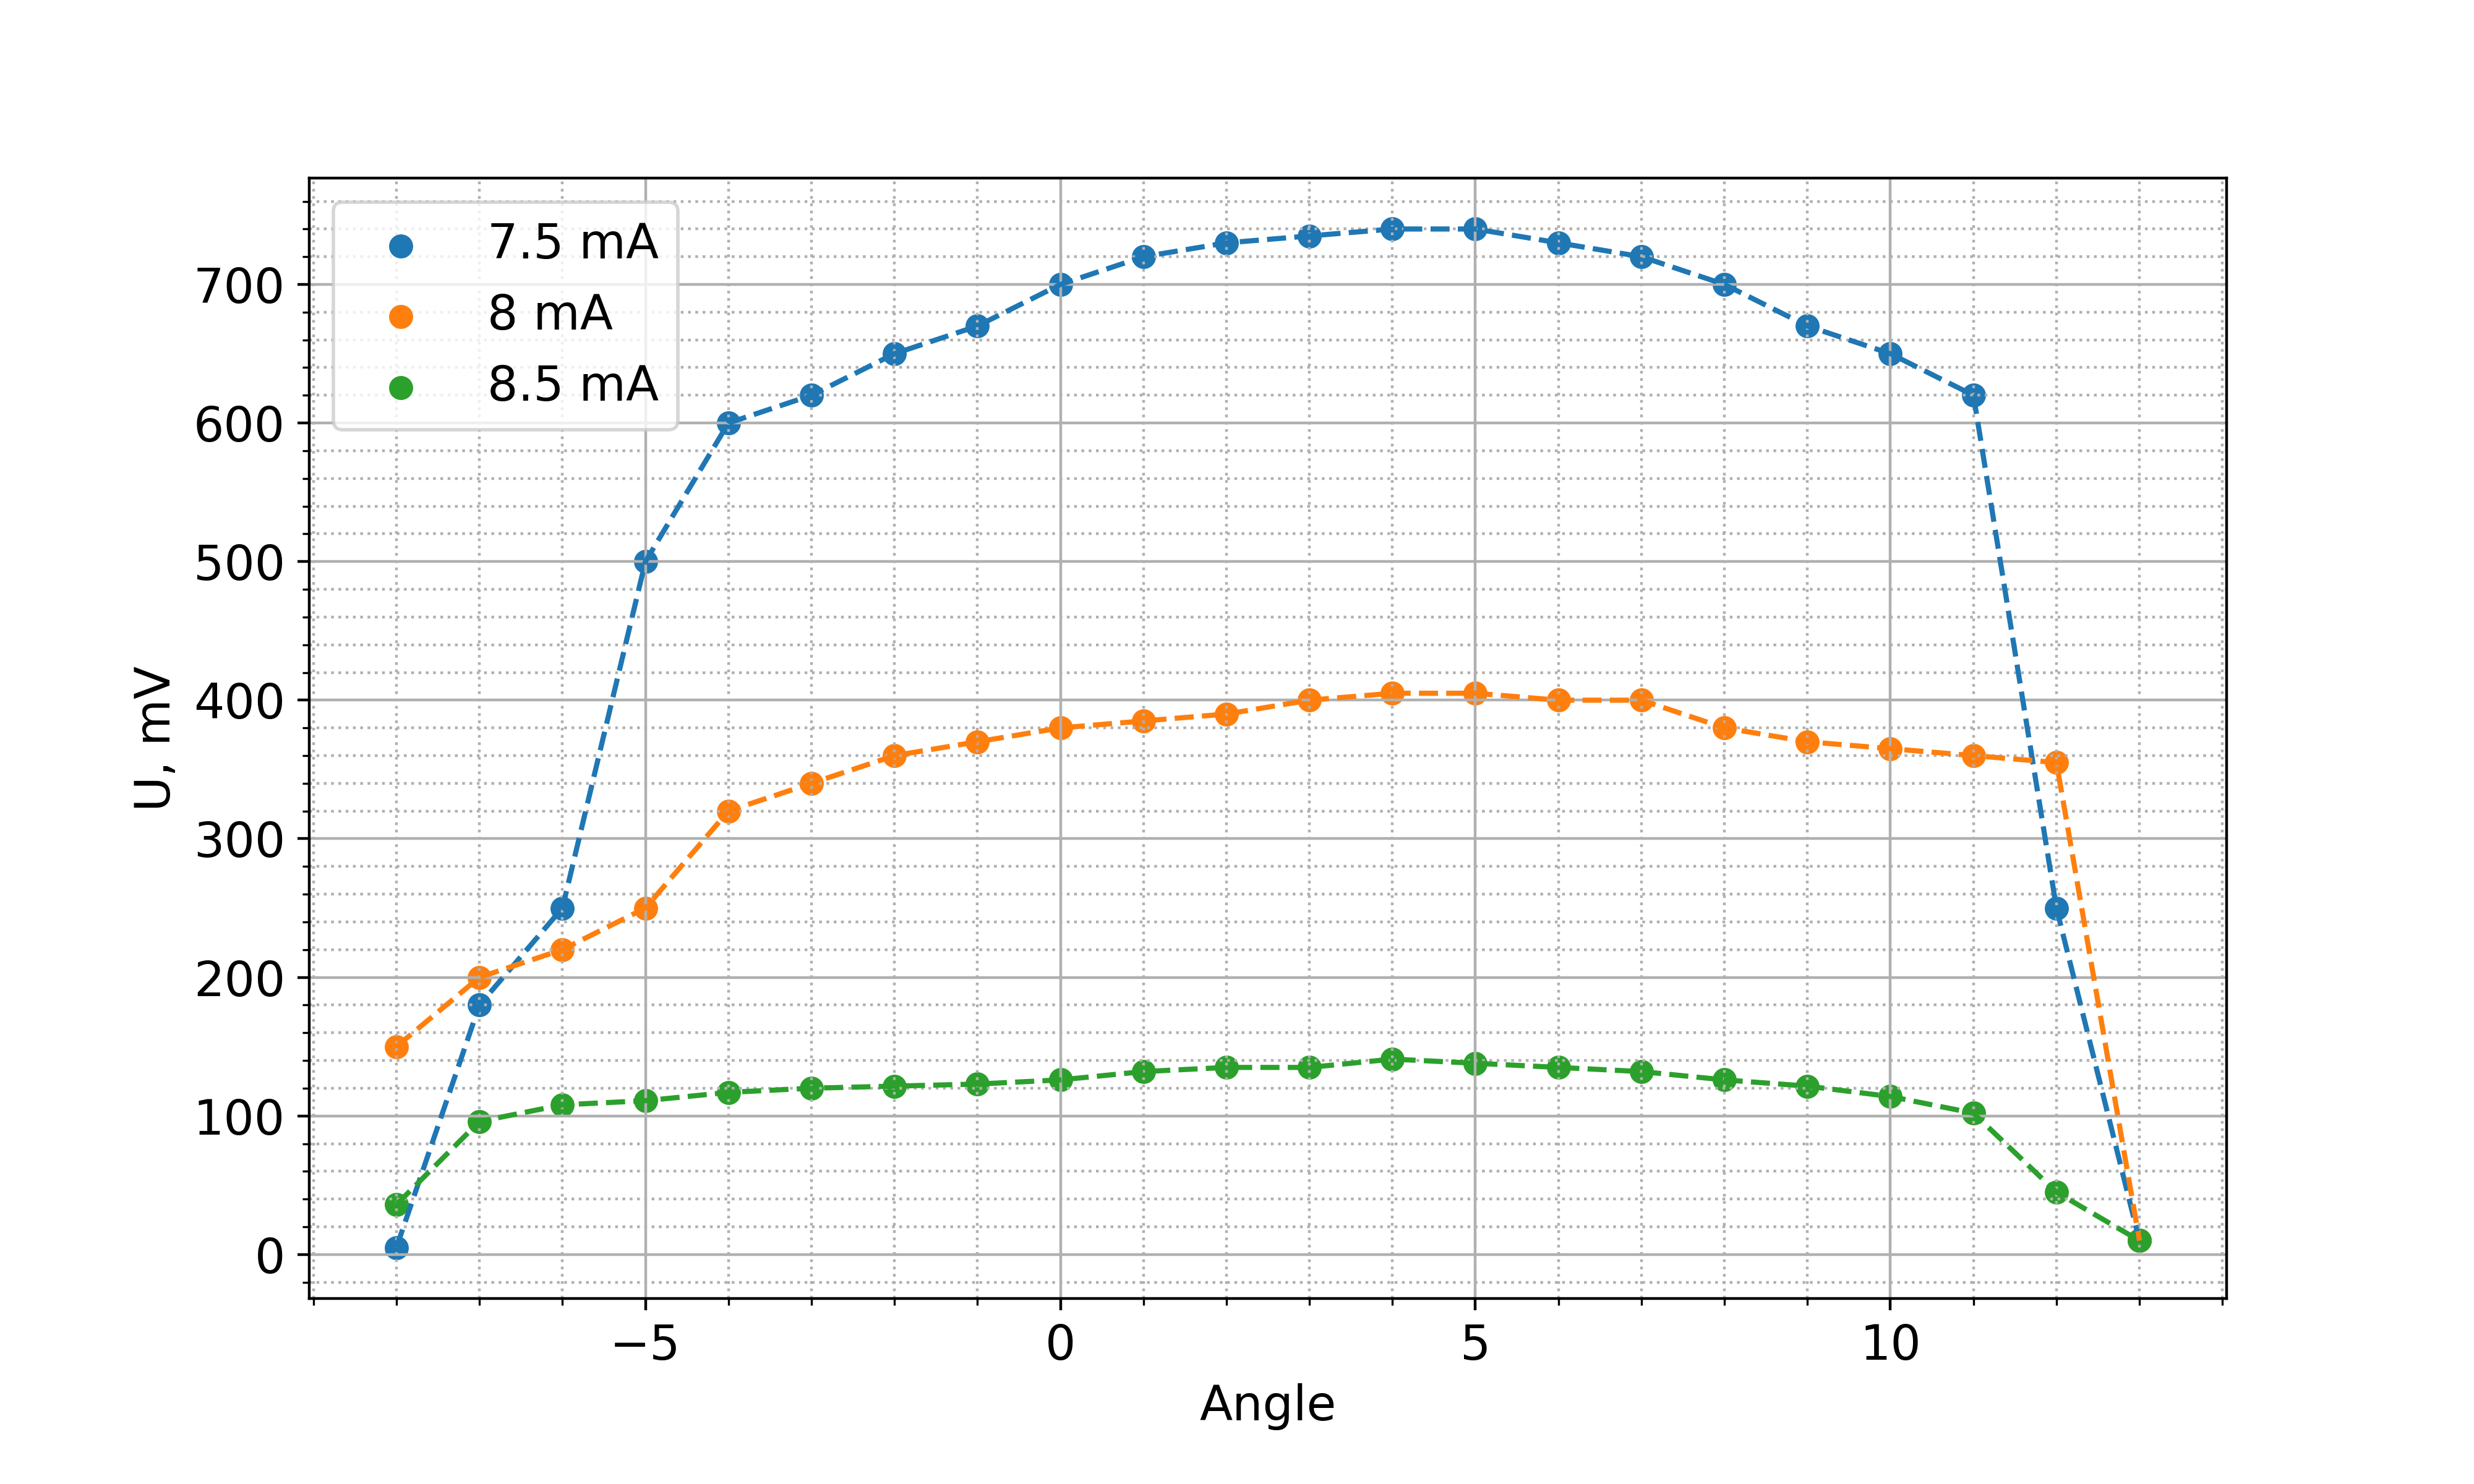
\includegraphics[scale=0.5]{g1.png}
        \caption{U(Angle)}
        \label{g1}
    \end{center}
\end{figure}






\end{document}